\documentclass[tikz,border=10pt]{article}
\title{Bell's spaceship paradox}
\author{Hans Halvorson}
\date{\today}
\usepackage{pgfplots}
\pgfplotsset{compat=newest}

\usepackage{amsfonts}
\usepackage{amsthm}
\theoremstyle{definition}
\usepackage{amsthm}
\newtheorem*{question}{Question}
\newtheorem*{fact}{Fact}

\newcommand{\vecc}[1]{\overrightarrow{#1}}

\begin{document}

\maketitle

Consider the following sketch of the trajectories of the two
spaceships. We assume that Alice (green) and Bob (blue) receive the
instruction to accelerate at the same time in what was originally
their common reference frame. The red vector is tangent to Bob's
trajectory at the point $(\sqrt{2},1)$.

\bigskip \noindent 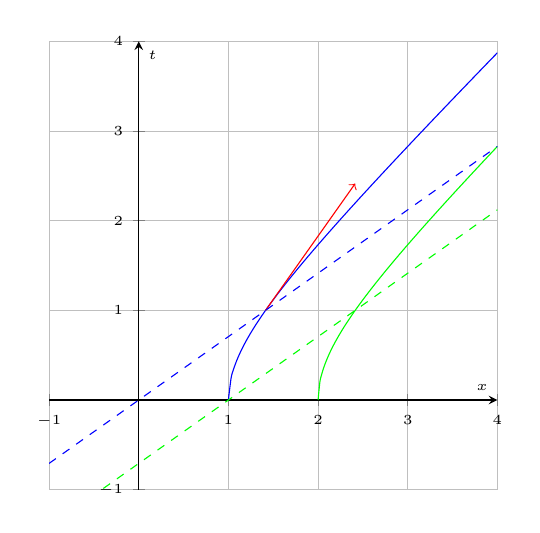
\begin{tikzpicture}
    \begin{axis}[
        axis lines=middle,
        xlabel={$x$},
        ylabel={$t$},
        xlabel style={font=\tiny}, % Makes the x-axis label smaller
        ylabel style={font=\tiny}, 
        xmin=-1, xmax=4,
        ymin=-1, ymax=4,
        grid=both,
        grid style={line width=.1pt, draw=gray!10},
        major grid style={line width=.2pt,draw=gray!50},
        axis equal image,
        legend pos=north west,
        tick label style={font=\tiny}, 
    ]
    % Original hyperbola (positive y values only)
    \addplot[domain=1:4, samples=100, smooth, blue] {sqrt(x^2 - 1)};

    % Shifted hyperbola (positive y values only)
    \addplot[domain=2:4, samples=100, smooth, green] {sqrt((x-1)^2 - 1)};

    % Tangent vector at x=2
    \draw[->, red] (axis cs:{sqrt(2)},1)--++(axis direction cs:1,{sqrt(2)});

    % Calculate slope
    \pgfmathsetmacro{\slope}{1/sqrt(2)}

    % Calculate y-intercept
    \pgfmathsetmacro{\yintercept}{1 - \slope*sqrt(2)}

    % Plot the line
    \draw[blue, dashed] (-1,{\slope*-1 + \yintercept}) -- (4,{\slope*4 + \yintercept}) node[right] {};

    \pgfmathsetmacro{\yinterceptNew}{1 - \slope*(1 + sqrt(2))}

    % Plot the new line
    \draw[green, dashed] (-1,{\slope*-1 + \yinterceptNew}) -- (4,{\slope*4 + \yinterceptNew}) node[right] { };
    \end{axis}
  \end{tikzpicture}

  \bigskip \noindent At each time (in the lab frame, or
  equivalently, according to the amount of elapsed proper time), Alice
  and Bob will have the same tangent vector, and so the same foliation
  into spatial hyperplanes. However, Alice and Bob will be located on
  different timeslices in this foliation.

For example, Bob reaches coordinate $(\sqrt{2},1)$ in the lab frame at
the same time that Alice reaches coordinate $(1+\sqrt{2},1)$. [In
fact, Alice's trajectory is just a translation by one unit to the
right --- in the lab frame --- of Bob's trajectory.] Their common
foliation consists of lines with slope $1/\sqrt{2}$. However, Bob lies
on the line that has $y$-intercept $0$ while Alice lies on the line
that has $y$-intercept $-1/\sqrt{2}$.

\begin{fact} The spacetime distance between Alice and Bob does not
  change. To be more precise, if $a(t)$ represents Alice's position at
  time $t$ and $b(t)$ represents Bob's position at time $t$, then
  $d(a(t),b(t))=1$ for all $t\in\mathbb{R}^+$. \end{fact}

This follows directly from the fact that Alice's trajectory is simply
a constant shift of Bob's trajectory.

\begin{fact} The point $(1,0)=b(0)$ lies on Alice's simultaneity
  surface at all times. What's more, $\vecc{b(0)a(t)}$ is spacelike,
  and $\| \vecc{b(0)a(t)}\| =1$ for all $t\in\mathbb{R}^+$. \end{fact}

\begin{proof} Note that the hyperbola $\{ (x,t):x^2-t^2=1\}$ consists of points
  that are Minkowski distance $1$ from $(0,0)$. Hence the hyperbola
  $\{ (x,t):(x-1)^2-t^2=1\}$ consists of points that are distance $1$
  from $(1,0)$. 
\end{proof}


\begin{question} What is the orthogonal (temporal) distance between
  Alice and Bob's hypersurfaces at time $t$? \end{question}
  
\end{document}


%%% Local Variables:
%%% mode: latex
%%% TeX-master: t
%%% End:
